\documentclass[10pt]{article}

\usepackage{fullpage}
\usepackage{longtable}
\usepackage[pdftex]{graphicx}
\DeclareGraphicsExtensions{.pdf,.jpg}

% no numbers, etc
\pagestyle{empty}

\begin{document}

{\bf Homework 4} \hfill {\raggedleft Thomas Torsney-Weir}

%Each homework problem goes here
\begin{enumerate}
\item % wumpus
  \begin{description}
  \item[Wumpus Net] In {\tt wumpus\_net.bif}
  \item[CPT Rationale] 
    There are 100 squares so the prior probability of a wumpus is 0.01.

    If the wumpus is in a next square then there is always a stench so
    the probability of a stench given the wumpus is always 1.  However, 
    there may be a stench even if the wumpus isn't in a particular square
    since it may be in any one of three remaining surrounding squares.  So
    the probability of no stench given no wumpus is $0.99^4$.  Here is the
    CPT table for each of the stench variables: \\
    \begin{tabular}{|c|c|c|}
    \hline
    $W$  &  $P(s)$ & $P(\neg s)$ \\ \hline
    $t$  &  1.0    & 0.0 \\
    $f$  &  0.0394 & 0.9606 \\
    \hline
    \end{tabular}

  \item[Console Dump] In {\tt wumpus\_net.console}
  \end{description}

\item % med test
  Probability table: \\
  \begin{tabular}{|c|c|c|}
  \hline
              & P($x |$ Disease) & P($x | \neg$ Disease) \\ \hline
  Test        & 0.91             & 0.09                  \\ \hline
  $\neg$ Test & 0.06             & 0.94                  \\ 
  \hline
  \end{tabular}

  \begin{eqnarray*}
  P(Disease | x)    & = & \alpha \langle P(Test | Disease) P(Disease),
                             P(Test | \neg Disease) P(\neg Disease) \rangle \\
                    & = & \alpha \langle 0.91 * 0.02, 0.09 * 0.98 \rangle \\
                    & = & \alpha \langle 0.0182, 0.0882 \rangle \\
  \alpha            & = & 9.3985 \\
  P(Disease | Test) & = & 0.1710527
  \end{eqnarray*}

\item % 13.6 (p 489)
  \begin{enumerate}
  \item % a
    $0.108 + 0.012 + 0.016 + 0.064 = 0.2$
  \item % b
    $0.108 + 0.012 + 0.072 + 0.008 = 0.2$
  \item % c
    $0.108 + 0.012 = 0.12$
  \item % d
    $0.108 + 0.012 + 0.072 + 0.016 + 0.064 + 0.144 = 0.416$
    
  \end{enumerate}

\item % simple bayes net
  \begin{eqnarray*}
  P(d | a) & = & \sum_b \sum_c P(B | a)  P(C | a)  P(d | B, C) \\
           & = & P(b | a)  P(c | a)  P(d | b,c) + \\
           &   & P(b | a)  P(\neg c | a) P(d | b, \neg c) + \\
           &   & P(\neg b | a) P(c | a) P(d | \neg b, c) + \\
           &   & P(\neg b | a) P(\neg c | a) P(d | \neg b, \neg c) \\
           & = & 0.2 * 0.7 * 0.3 + 0.2 * 0.3 * 0.25 + \\
           &   & 0.8 * 0.3 * 0.1 + 0.8 * 0.3 * 0.35 \\
           & = & 0.197
  \end{eqnarray*}
\item % 14.1 a-d (p 533)
  \begin{enumerate}
  \item % a
    \ \\
    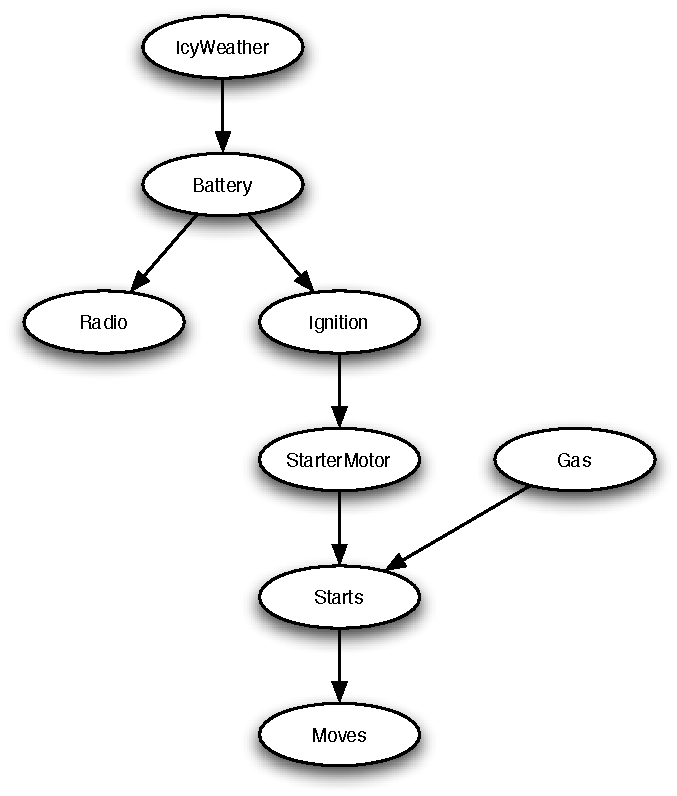
\includegraphics{5a_car.pdf}

  \item % b
    \begin{description}
    \item[IcyWeather]
      \ \\
      \begin{tabular}{|c|c|}
      \hline
      $P(IW)$ & $P(\neg IW)$ \\ \hline
      0.1     & 0.9 \\
      \hline
      \end{tabular}

    \item[Battery]
      \ \\
      \begin{tabular}{|c|c|c|}
      \hline
      $IW$ & $P(B)$ & $P(\neg B)$ \\ \hline
      $t$  & 0.7    & 0.3 \\
      $f$  & 0.9    & 0.1 \\
      \hline
      \end{tabular}

    \item[Radio]
      \ \\
      \begin{tabular}{|c|c|c|}
      \hline
      $B$ & $P(R)$ & $P(\neg R)$ \\ \hline
      $t$  & 0.85    & 0.15   \\
      $f$  & 0.0    & 1.0 \\
      \hline
      \end{tabular}

    \item[Ignition]
      \ \\
      \begin{tabular}{|c|c|c|}
      \hline
      $B$ & $P(I)$ & $P(\neg I)$ \\ \hline
      $t$  & 0.95   & 0.05   \\
      $f$  & 0.005  & 0.995 \\
      \hline
      \end{tabular}

    \item[StarterMotor]
      \ \\
      \begin{tabular}{|c|c|c|}
      \hline
      $I$ & $P(SM)$ & $P(\neg SM)$ \\ \hline
      $t$  & 0.95   & 0.05   \\
      $f$  & 0.001  & 0.999 \\
      \hline
      \end{tabular}

    \item[Gas]
      \ \\
      \begin{tabular}{|c|c|}
      \hline
      $P(G)$ & $P(\neg G)$ \\ \hline
      0.5    & 0.5 \\
      \hline
      \end{tabular}

    \item[Starts]
      \ \\
      \begin{tabular}{|c|c|c|c|}
      \hline
      $SM$ & $G$ & $P(S)$ & $P(\neg S)$ \\ \hline
      $t$  & $t$ & 0.89   & 0.11 \\
      $t$  & $f$ & 0.02   & 0.98 \\
      $f$  & $t$ & 0.01   & 0.99 \\
      $f$  & $f$ & 0.0    & 1.0 \\
      \hline
      \end{tabular}

    \item[Moves]
      \ \\
      \begin{tabular}{|c|c|c|}
      \hline
      $S$ & $P(M)$ & $P(\neg M)$ \\ \hline
      $t$  & 0.75   & 0.25   \\
      $f$  & 0.20   & 0.8 \\
      \hline
      \end{tabular}
    \end{description}
  \item % c
    $2^n = 2^8 = 256$
  \item % d
    16
  \item % e
    The noisy-AND distribution has probability 1 if and only if all its 
    parents are true.  This is in contrast to the noisy-OR distribution 
    which has probability 0 if and only if all its parents are false.
  \end{enumerate}

\item % 14.2 a,c,d (p 533-4)
  \begin{enumerate}
  \item % a
    \ \\
    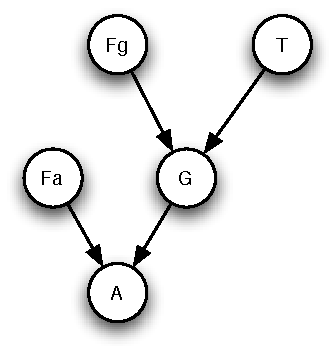
\includegraphics{6a_nuclear.pdf}

  \item % c
    \ \\
    \begin{tabular}{|c|c|c|c|}
    \hline
    $F_G$ & $T$ & $P(G=h)$ & $P(G=n)$ \\ \hline
    $t$   & $h$ & $x$      & $1 - x$ \\
    $t$   & $n$ & $1 - x$  & $x$ \\
    $f$   & $h$ & $1 - y$  & $y$ \\
    $f$   & $n$ & $y$      & $1 - y$ \\
    \hline
    \end{tabular}

  \item % d
    \ \\
    \begin{tabular}{|c|c|c|c|}
    \hline
    $F_A$ & $G$ & $P(A)$ & $P(\neg A)$ \\ \hline
    $t$   & $h$ & 1.0    & 0.0 \\
    $t$   & $n$ & 0.0    & 1.0 \\
    $f$   & $h$ & 0.0    & 1.0 \\
    $f$   & $n$ & 0.0    & 1.0 \\
    \hline
    \end{tabular}

  \end{enumerate}

\item % 14.3 a-b (p 534)
  \begin{enumerate}
  \item % a
    They are all valid.
    
  \item % b
    The best would be network ii.  This is because the out of focus variables
    ony affect the measurements.  It would also be much easier to determine
    a measurement based on the number of stars rather than the number of
    stars based on a measurement.
  \end{enumerate}

\end{enumerate}

\end{document}

